\documentclass[12pt,a4paper]{book}
\usepackage{datetime}
\usepackage{graphicx}
\usepackage[margin=1.5cm]{geometry}
\usepackage{csvsimple}
\usepackage{longtable}
\begin{document}
\setlength{\parindent}{0cm}

\begin{titlepage}
  \begin{center}
    \textsc{\LARGE Digital Lab Notebook of Kevin Murray}\\[1.5cm]
    \textsc{\Large Honours Project, 2013}\\[0.5cm]
    \textit{Jointly supervised by Justin Borevitz and Barry Pogson}\\
    \vfill
    \textit{Last updated at \currenttime on \today}\\
  \end{center}
\end{titlepage}

\chapter*{Mon 2012-12-03}
  \section*{Initial Harvest of Keng's RIX lines}
    \subsection*{Aim}
      Harvest lines before the 1 week repeated HL stress experiment.
    \subsection*{Method}
      \begin{itemize} \itemsep1pt \parskip0pt \parsep0pt
        \item Tissue was harvested into a 96 well tray of 8-strip $\approx$ 1mL tubes
        \item Single leaves were placed into the tubes, and snap frozen in liquid nitrogen.
      \end{itemize}
    \subsection*{Results}
      The following table details the collection, including the plate layout
      \csvautolongtable{./2012-12/20121203-InitialHarvest.csv}
      \emph{Attachments:}
      \begin{itemize} \itemsep1pt \parskip0pt \parsep0pt
        \item \verb+./2012-12/20121203-harvest-pictures.tar.bz2+ \hfill
          MD5SUM:2843946f8cae888a60dcd2226feb874f
      \end{itemize}

\chapter*{Mon 2012-12-10}
  \section*{Final Harvest of Keng's RIX lines}
    \subsection*{Aim}
      Harvest lines after 1 week of HL stress.
    \subsection*{Method}
      \begin{itemize} \itemsep1pt \parskip0pt \parsep0pt
        \item An Eppendorf 1.2mL deep well plate was placed on dry ice for $\approx$ 10 minutes before
          sampling to allow to cool.
        \item Whole leaves were excised and placed into 1.2mL Eppendorf 96 deep well plate.
        \item Where possible, the largest mature leaf was taken. In some cases, this was hard to
          determine, so the youngest of the fully-expanded leaves was taken (as this was generally
          also the largest leaf). Some plants were very small, and had only juvenile leaves, in which
          case the largest juvenile leaf was taken.
      \end{itemize}
    \subsection*{Results}
    The following table describes the plate layout.
    \csvautolongtable{./2012-12/20121210-FinalHarvest.csv}
    \emph{Attachments:}
    \begin{itemize} \itemsep1pt \parskip0pt \parsep0pt
      \item \verb+./2012-12/20121210-harvest-photos.tar.bz2+ \hfill MD5SUM:40dae2cad3babaa3c32f0d35a9d9442c
    \end{itemize}

\chapter*{Mon 2013-01-14}
  \section*{MAKE: Washed Ball Bearings}
    \subsection*{Method}
      \begin{itemize} \itemsep1pt \parskip0pt \parsep0pt
        \item Aliquot approx 15mL of 3mm diameter steel ball bearings into 50mL falcon tube
        \item Add clean 100\% ethanol
        \item Vortex for $\approx$ 5 minutes
        \item Remove ethanol, wash beads with milliQ or sterile water
        \item Dry in fume cupboard overnight
      \end{itemize}

  \section*{TissueLyser grinding of practice samples}
    \subsection*{Aims}
      To grind tissue from the excess tissue of Keng's RIX lines collected on 3/12/12.
    \subsection*{Method}
      \begin{itemize} \itemsep1pt \parskip0pt \parsep0pt
        \item Remove pre-frozen TissueLyser blocks from -80 freezer.
        \item Add one cleaned bead to each Eppendorf tube (beads were not pre-cooled)
        \item Pour LN$_2$ into the TissueLyser block
        \item Add Eppys with beads and sample, and run for 3x 1min runs at 29Hz
        \item Replace samples in -80
      \end{itemize}

\chapter*{Mon 2013-01-21}
  \section*{Quantification of RNA samples}
    \subsection*{Aim}
      \begin{itemize} \itemsep1pt \parskip0pt \parsep0pt
        \item Determine qty of RNA in previously extracted samples
      \end{itemize}

    \subsection*{Method}
      \begin{itemize} \itemsep1pt \parskip0pt \parsep0pt
        \item Nanodropped RNA extraction from 15/1/13??
        \item Standard protocol, used sterile milliQ water as blank.
      \end{itemize}

    \subsection*{Result}
      \begin{itemize} \itemsep1pt \parskip0pt \parsep0pt
        \item Of the 14 samples, 10 had reasonable amounts of RNA, and 260/280 ratios were above 1.8 in all but one case.
        (see \verb+./2013-01/20130121-PracticeRNASamples.ods+)
      \end{itemize}

    \subsection*{Attachments}
      \begin{itemize} \itemsep1pt \parskip0pt \parsep0pt
        \item \verb+./2013-01/20130121-PracticeRNAExtractionSamples.csv+
        \item \verb+./2013-01/20130121-PracticeRNAExtractionSamples.ndv+
        \item \verb+./2013-01/20130121-PracticeRNASamples.ods+
      \end{itemize}

  \section*{MADE: 10x MOPS Solution}
    \emph{Method}
    \begin{itemize} \itemsep1pt \parskip0pt \parsep0pt
      \item Add 41.8g RNA only MOPS to beaker
      \item Add ~450mL DEPC H2O, mix w/ stirrer bar on mag stirrer
      \item Add 26.6mL 3M Sodium Acetate (0.22um Filtered before use)
      \item Add 10mL RNA only 0.5M EDTA
      \item pH to 7 with 5M NaOH
      \item Top up to 500 mL with DEPC H2O
      \item Use 10ml per 100mL MOPS gel
    \end{itemize}

  \section*{MADE: RNA Denaturing Gel (MOPS)}
    \emph{Method}
    \begin{itemize} \itemsep1pt \parskip0pt \parsep0pt
      \item Melt 1g RNAase-free Agarose in 72ml DEPC H2O
      \item Add 10mL 10x MOPS
      \item Add 18mL 37\% Formaldehyde
      \item Pour in RNA-only gel tank, previously washed with 0.5\% SDS and RNAase-zap
    \end{itemize}

\chapter*{Tue 2013-01-22}
  \section*{Denature RNA for RNA gels}
    \subsection*{Method}
      \begin{itemize} \itemsep1pt \parskip0pt \parsep0pt
        \item Dilute RNA to 100ng/µL
        \item Add RNA gel loading buffer (Obtained from Pete Crisp)
        \item Incubate at 65 degrees for 10 minutes. The samples were incubated for 10 minutes on the evening of
          2013-01-21, but the gels were not run until 2013-01-22, so they were denatured for a further 2 minutes at 65
          degrees
      \end{itemize}

  \section*{TBE Gel}
    \subsection*{Aim}
      \begin{itemize} \itemsep1pt \parskip0pt \parsep0pt
        \item To compare TBE and denaturing/MOPS gels for RNA
      \end{itemize}

    \subsection*{Method}
      \begin{itemize} \itemsep1pt \parskip0pt \parsep0pt
        \item Dissolve 1g RNAase-free Agarose in 90mL DEPC water
        \item Add 10mL RNAase-free TBE (prepared using DEPC Water, obtained from Pete Crisp)
        \item Pour in RNA-only gel tank, previously washed with 0.5\% SDS or RNAase-zap
        \item Then, load denatured samples, and run in RNAase-free 1x TBE
        \item Run at $\approx$ 80V, $\approx$ 40-50mA for $\approx$ 1.75h
        \item Stain gel in 0.5ug/ml Ethidium Br in DEPC water?? for 10 min on orbital shaker, and photograph.
      \end{itemize}

    \subsection*{Result}
      \begin{figure}[h!]
        \caption{TBE Gel of Practice RNA samples, 2013-01-22}
        \centering
          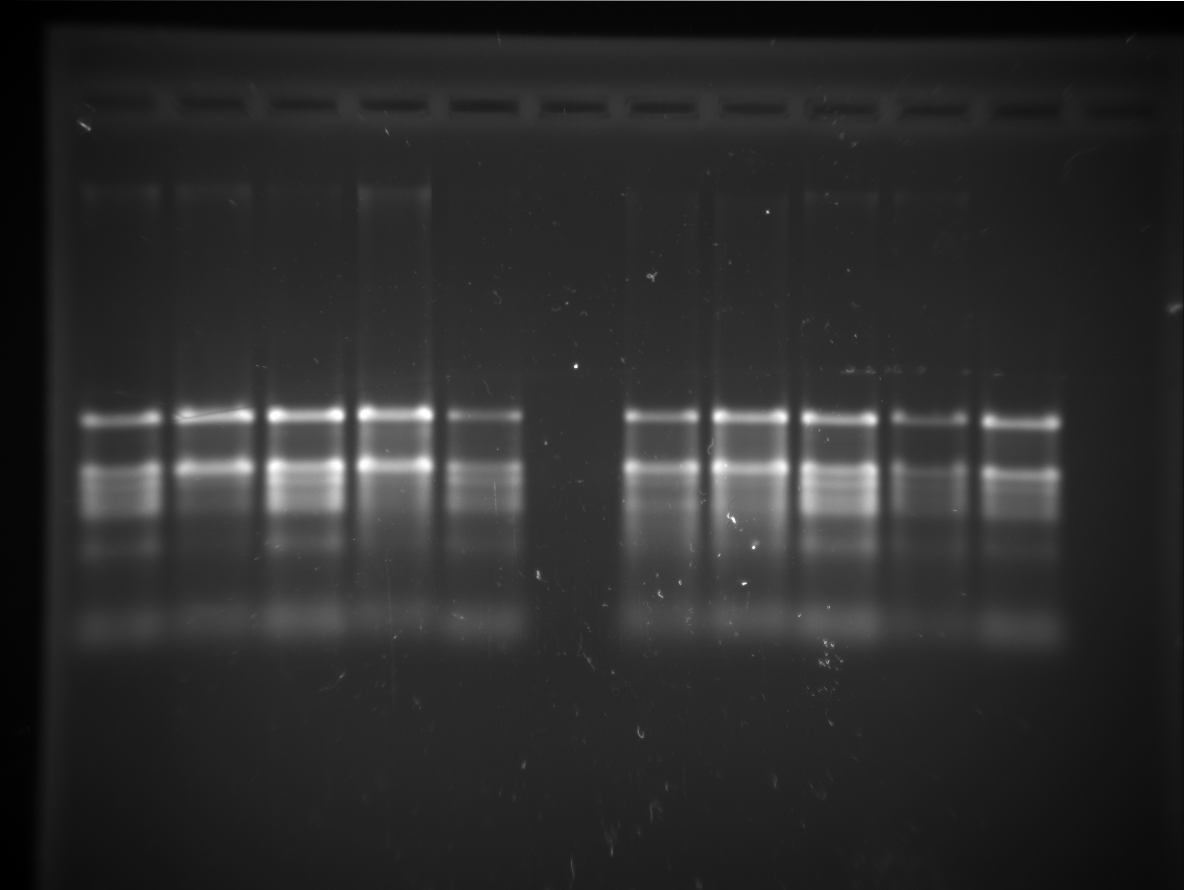
\includegraphics[width=0.9\textwidth]{./2013-01/20130122-PracticeRNATBE}
        \label{fig:20130122-PracticeRNATBE}
      \end{figure}
      See Figure \ref{fig:20130122-PracticeRNATBE} below.\\
      Gel indicates some degradation of RNA, however most samples are OK. Sample order is (left to right) A2, A3, A5,
      A6, A7, B3, B5, B7. A7 appears to have no RNA, although this is probably a mis-loading error. Overall, the TBE gel
      appears to be of more use than the MOPS gel.\\

  \section*{MOPS gel}
    \subsection*{Aim}
      \begin{itemize} \itemsep1pt \parskip0pt \parsep0pt
        \item Determine quality of RNA and Compare MOPS with TBE for RNA gels
      \end{itemize}

    \subsection*{Method}
      \begin{itemize} \itemsep1pt \parskip0pt \parsep0pt
        \item Load samples after denaturing as above. Sample order is (left to right) A2, A3, A5, A6, A7, B3, B5, B7.
        \item Run gel in RNAase free 1x MOPS at $\approx$ 80V, $\approx$ 100mA for $\approx$ 1.75h as per TBE gel above.
        \item Stain gel in 0.5ug/ml Ethidium Br in DEPC water?? for 10 min on orbital shaker.
        \item De-stain on orbital shaker gel in 1x MOPS, and photograph. Gel disintegrated whilst de-staining.
      \end{itemize}

    \subsection*{Results}
      \begin{figure}[h!]
        \caption{MOPS Gel of Practice RNA samples, 2013-01-22}
        \centering
          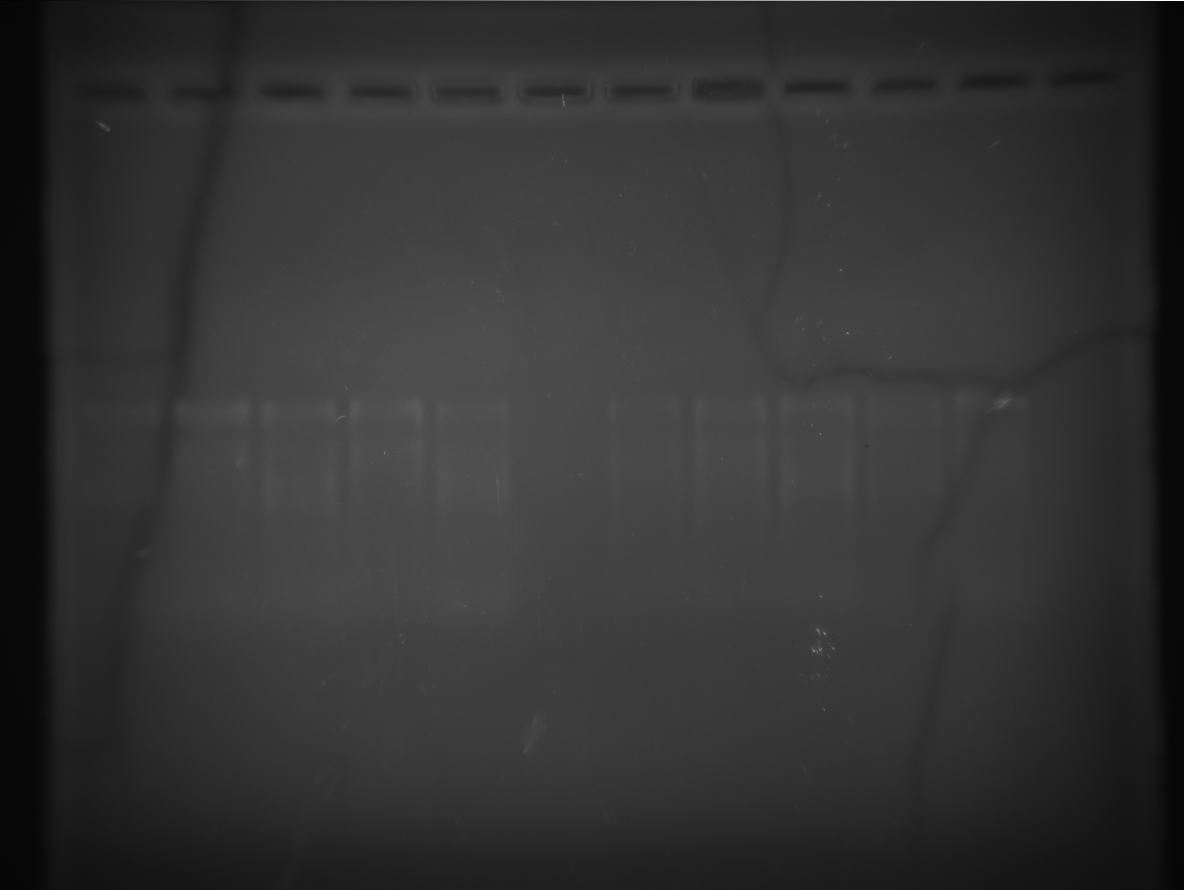
\includegraphics[width=0.9\textwidth]{./2013-01/20130122-PracticeRNADenaturedMOPS}
        \label{fig:20130122-PracticeRNADenaturedMOPS}
      \end{figure}

      \begin{figure}[h!]
        \caption{MOPS Gel of Practice RNA samples, 2013-01-22. Contrast adjusted.}
        \centering
          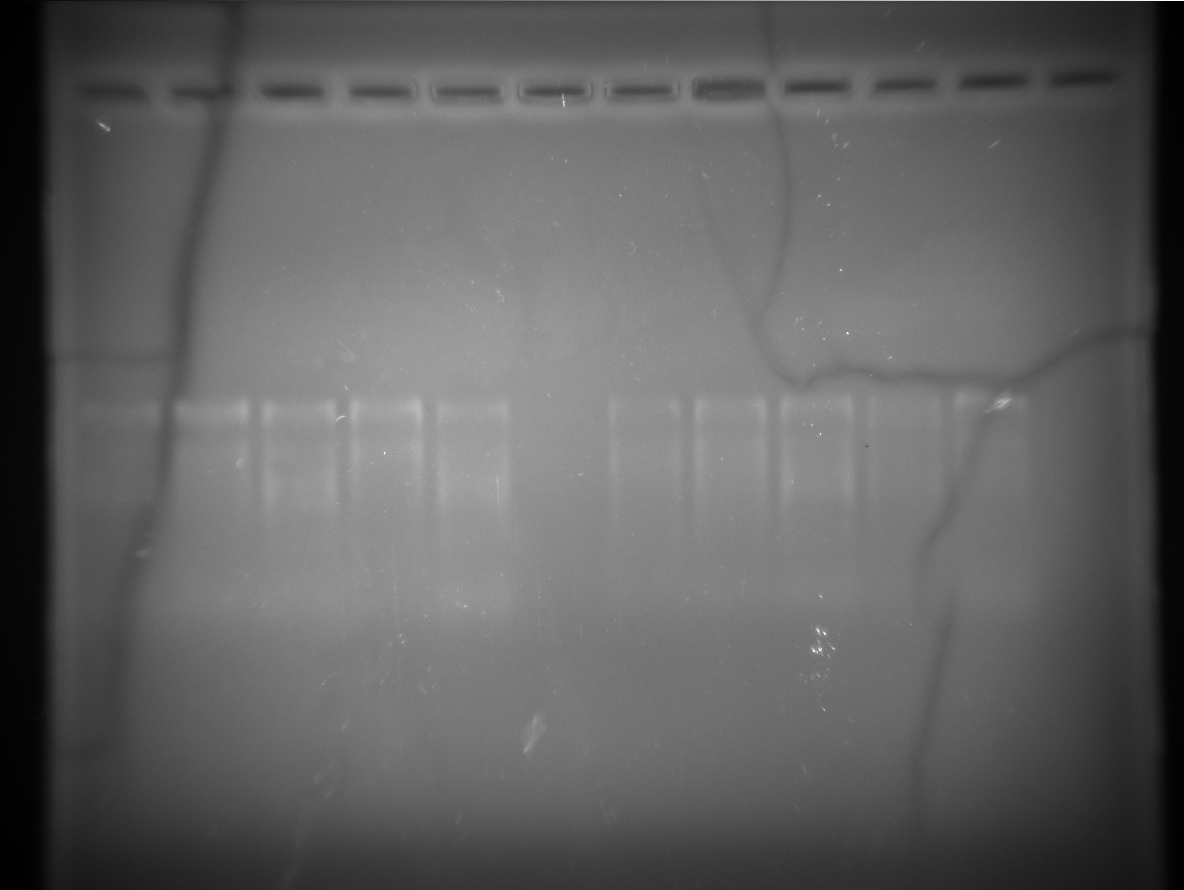
\includegraphics[width=0.9\textwidth]{./2013-01/20130122-PracticeRNADenaturedMOPS-HighContrast}
        \label{fig:20130122-PracticeRNADenaturedMOPS-HighContrast}
      \end{figure}

      See Figures \ref{fig:20130122-PracticeRNADenaturedMOPS} and
      \ref{fig:20130122-PracticeRNADenaturedMOPS-HighContrast}\\
      Mops gel confirms that the RNA was of reasonable quality. The MOPS gel appears to be of less use than the TBE
      gel.\\

\chapter*{Tue 2013-01-29}
  \section*{Seed Stock Levels}
    The stocks of Joost's RIX set were checked. Seed lines were classified as having either plenty
    (+), limited(?) or no (-) seed. The levels of each line are shown in the table below.
    \csvautolongtable{./2013-01/20130129-SeedStockLevels.csv}

\chapter*{Thu 2013-02-07}
  \section*{Prepare Trays for Planting}
    Trays were filled with steamed seed raising mix, with 1mL/L Osmocote® added and mixed before
    dispensing. Trays were filled by pouring potting mix over tall 5cm square pots, and compacting
    it with hands. 41 trays of 24 and one tray of 20 pots were made.\\
    Once trays were made, they were watered with $\approx$ 1.5L RO water, containing $\approx$ 1mL/L
    AzaMax™, covered with cling film and stored at 4 degrees C.

\chapter*{Fri 2013-02-08}
  \section*{Planting of RIX lines}
    \subsection*{Aim:}
      Plant (ideally) 9 plants of each of the RIX lines, for the experiment Keng and I will
      conduct
    \subsection*{Method:}
      Seeds were planted in pre-prepared trays, by shaking from a piece of paper. Either 6 or 12
      plants of each line, and some mutants, were planted in contiguous blocks. Once planted, trays
      were sprayed with a small amount of water and labelled by row, i.e. each row of plants
      consisted of one genotype, and only one pot was labelled per row. Plants were not randomised at
      this point. If the tray was dry, approx 0.5-1L of RO water was added.\\
      The following table describes the lines which were planted. 12 plants of each line were
      planted, unless otherwise stated in the ``Qty'' columns below. From now on, lines will be
      referred to by their number in the following table. \label{20130208-linestable}
      \csvautolongtable{./2013-02/20130208-KMPlantedLines.csv}

\chapter*{Thu 2013-02-14}
  \section*{Sun and Shade Spectra}
    \subsection*{Aim}
      Measure specta from natural sun and natural shade at midday
    \subsection*{Method}
      \begin{itemize} \itemsep1pt \parskip0pt \parsep0pt
        \item John Evan's spectroradiometer was used
        \item Measure every nm from 400 to 800
        \item Measurements taken at approx 12:30-1pm
        \item Measure clear, unobstructed sun with no clouds in quadrangle between forrestry,
          geography and Robertson buildings, ANU.
        \item Measure shade under elm tree in same location
        \item Calculations made by Pip Wilson, yielded umol photon per square meter per second per
          nanometer measures of intesnity. (see attached xls spreadsheet).
      \end{itemize}
    \subsection*{Results}
      Overall PAR integrations were 38.0 and 1809.5 uE for shade and sun respectively.\\
      Spectra detailed in:
      \begin{itemize} \itemsep1pt \parskip0pt \parsep0pt
          \item \verb+20130214-shade and sun spectra.xlsx+\\
            MD5SUM db67505144fbd20ecc317a494f80ecde
          \item \verb+20130214-SunShadeSpectra.csv+\\
            MD5SUM 56003985e19111288384dcd5f4dc51f1
      \end{itemize}

\chapter*{Fri 2013-03-01}
  \section*{Creation of Solarcalc files}
    \subsection*{Aim:}
      Generate the solar calc files which will be used to control the conviron growth cabinents and
      heliospectra lights for the duration of the latter part of the experiment.
    \subsection*{Method}
      \begin{itemize} \itemsep1pt \parskip0pt \parsep0pt
        \item SolarCalc version 2013 Feb C (zip file MD5SUM: 0b2b456771eb44ed1fa8ed1a087bfbd0) was
          used.
        \item Location: Temora
        \item Min Temp: 5 C
        \item Max Humid.: 80
        \item Start Date: 1/9/12
        \item End Date: 31/12/12
        \item Shading: 0
        \item LED Ratios: 7.74 6.16 5.98 5.64 7.35 1.00 5.45
        \item 2010 weather
      \end{itemize}
    \subsection*{Results}
      \begin{itemize} \itemsep1pt \parskip0pt \parsep0pt
        \item Solarcalc output:\\
          \verb+./2013-03/20130301-KMTemora2012Sep01_A_LED-Normalised.csv+ \\
          MD5sum b1dee0ba373a1e74956dd5c8d3ccce38
        \item Solarcalc preferences file:\\
          \verb+./2013-03/20130301-KMTemora2012Sep01_A_LED-Normalised_prefs.srp+ \\
          MD5SUM d01fcc5ae9ad8fba07bd9b9512c82857
      \end{itemize}

\chapter*{Thu 2013-03-05}
  \section*{Creation of Better Normalised Shaded Solarcalc files}
    \subsection*{Aim:}
      Generate the solar calc files which will be used to control the conviron growth cabinents and
      heliospectra lights for the duration of the latter part of the experiment.
    \subsection*{Method}
      \begin{itemize} \itemsep1pt \parskip0pt \parsep0pt
        \item SolarCalc version 2013 Feb C (zip file MD5SUM: 0b2b456771eb44ed1fa8ed1a087bfbd0) was
          used.
        \item Location: Temora
        \item Min Temp: 10 C
        \item Max Humid.: 70
        \item Start Date: 1/9/12
        \item End Date: 31/12/12
        \item Shading: 0 and 45\%
        \item LED Ratios: 1.29 1.03 .94 1.22 0.17 .91
        \item 2010 weather
      \end{itemize}
    \subsection*{Results}
      Solarcalc outputs:
      \begin{itemize} \itemsep1pt \parskip0pt \parsep0pt
          \item \verb+./2013-03/20130305-Temora2012Sep01_45shade_2010weather_LED-BetterNormalised.csv+\\
            ddff182b78d1fe10e662fb827a179804
          \item \verb+./2013-03/20130305-Temora2012Sep01_0shade_2010weather_LED-BetterNormalised.csv+\\
            d41d8cd98f00b204e9800998ecf8427e
      \end{itemize}
      Solarcalc preferences files:
      \begin{itemize} \itemsep1pt \parskip0pt \parsep0pt
          \item \verb+./2013-03/20130305-Temora2012Sep01_0shade_2010weather_LED-BetterNormalised.srp+\\
            9e800ba2b31a5346b37bc17127515d38
          \item \verb+./2013-03/20130305-Temora2012Sep01_45shade_2010weather_LED-BetterNormalised.srp+\\
            d40480b773fdaad8ecf9bd14a5d445ed
      \end{itemize}


\end{document}
